% Provenance (never printed): cycle 3 / 6e "La planete Terre" (water in the
% ground, groundwater, springs and wells; resource); see
% sources/book1/PROVENANCE.md. Book 1, grade 6, chapter 5.
% Vocabulary guard: "sediment" not before g7.4; the water cycle is recalled
% from the physics book (prose only).
\chapter{A água subterrânea}\label{ch:g6:water-underground}

Num dia quente de verão, os campos estão secos e os riachos estão baixos.
Mesmo assim, no pé de um morro, a água continua brotando do chão, fria e
limpa, como brotou o inverno todo, e enche um \omterm{def:g6:water-underground:spring}{poço} natural. Não chove há
semanas. De onde vem essa água, e como ela sai da \omterm{def:g3:stones-pebbles-sand:rock}{rocha}?

\begin{omfigure}
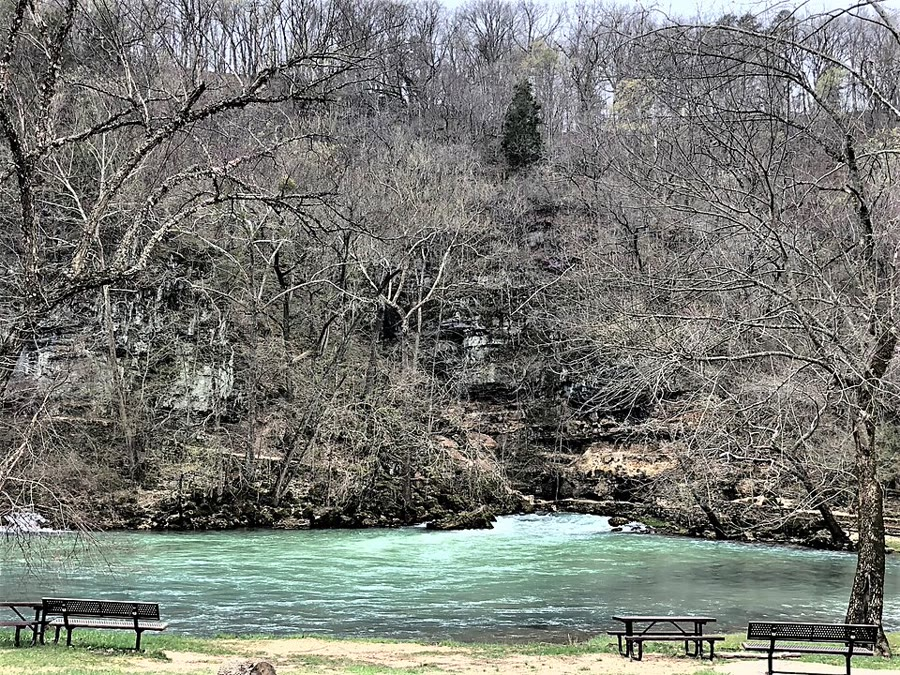
\includegraphics[width=0.72\linewidth]{images/book1/g6-big-spring.jpg}

{\small Uma \omterm{def:g6:water-underground:spring}{fonte} brota no pé de um paredão rochoso e enche um \omterm{def:g6:water-underground:spring}{poço}
natural: Big Spring, no Missouri (Estados Unidos). (Foto: Johnston9494,
CC BY-SA 4.0, via Wikimedia Commons.)}
% ledger: commons:big-spring
\end{omfigure}

\begin{recall}
Quase toda a água da Terra é \omterm{def:g2:water-on-earth:salt-fresh}{água salgada}; a \omterm{def:g2:water-on-earth:salt-fresh}{água doce} é uma pequena
parte, guardada sobretudo como gelo e embaixo do chão
(\cref{ch:g2:water-on-earth}). \omterm{def:g3:stones-pebbles-sand:rock}{Rochas} como o arenito e o calcário são
feitas de grãos ou de conchas grudados uns nos outros, enquanto a argila e
o folhelho são feitos de partículas muito finas
(\cref{ch:g6:rocks-and-minerals}). No livro de física, você seguiu a água
pelo ciclo da água: ela evapora dos \omterm{def:g2:water-on-earth:ocean}{mares}, se condensa em \omterm{def:g4:clouds-rain-snow:cloud}{nuvens} e cai de
volta como \omterm{def:g4:clouds-rain-snow:precipitation}{chuva} ou \omterm{def:g4:clouds-rain-snow:precipitation}{neve}.
\end{recall}

\section{A chuva se infiltra}

Quando a \omterm{def:g4:clouds-rain-snow:precipitation}{chuva} cai na terra, a água pode seguir três caminhos. Uma parte
evapora de volta para o ar. Uma parte corre pela superfície, encosta
abaixo, até os riachos e os \omterm{def:g1:landscapes-around-us:water}{rios}: é o \emph{escoamento superficial}. O
resto se infiltra no chão.

\begin{definition}[Infiltração]\label{def:g6:water-underground:infiltration}
A \emph{infiltração}\index{infiltracao@infiltração} é a penetração da água da \omterm{def:g4:clouds-rain-snow:precipitation}{chuva}, ou
da \omterm{def:g4:clouds-rain-snow:precipitation}{neve} derretida, no chão, através do solo e até as \omterm{def:g3:stones-pebbles-sand:rock}{rochas}.
\end{definition}

A quantidade de água que se infiltra depende do chão. Numa encosta
íngreme, num chão descoberto ou duro, numa rua ou num estacionamento, ou
quando o solo já está encharcado, a maior parte da água escorre. Numa
encosta suave, embaixo da grama e das árvores, num solo arenoso, uma parte
maior tem tempo de se infiltrar.

\begin{omfigure}
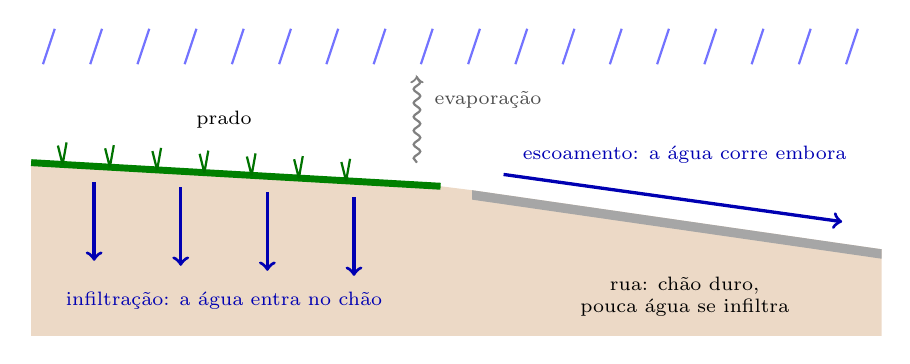
\begin{tikzpicture}[x=1cm, y=1cm]
  % rain
  \foreach \x in {0.3,0.9,...,10.5} \draw[blue!55, thick] (\x,3.9) -- (\x-0.15,3.45);
  % ground: field on the left (gentle), road and town on the right
  \fill[brown!30] (0,0) -- (0,2.2) -- (5.2,1.9) -- (5.6,1.85) -- (10.8,1.1) -- (10.8,0) -- cycle;
  \draw[green!50!black, line width=2.5pt] (0,2.2) -- (5.2,1.9);
  \fill[gray!70] (5.6,1.85) -- (10.8,1.1) -- (10.8,0.98) -- (5.6,1.73) -- cycle;
  \foreach \x in {0.4,1.0,...,4.6} \draw[green!45!black, thick] (\x,{2.2-0.058*\x}) -- ++(0.05,0.28) (\x,{2.2-0.058*\x}) -- ++(-0.06,0.24);
  % infiltration arrows in the field
  \foreach \x in {0.8,1.9,3.0,4.1} \draw[->, blue!70!black, very thick] (\x,{2.0-0.058*\x}) -- ++(0,-1.0);
  \node[font=\scriptsize, blue!70!black, align=center, fill=brown!30] at (2.45,0.45) {infiltração: a água entra no chão};
  % run-off on the road
  \draw[->, blue!70!black, very thick] (6.0,2.05) -- (10.3,1.45);
  \node[font=\scriptsize, blue!70!black, align=center] at (8.3,2.3) {escoamento: a água corre embora};
  \node[font=\scriptsize, align=center] at (8.3,0.5) {rua: chão duro,\\ pouca água se infiltra};
  \node[font=\scriptsize] at (2.45,2.75) {prado};
  % evaporation
  \draw[->, gray, thick, decorate, decoration={snake, amplitude=1.2pt, segment length=5pt}] (4.9,2.2) -- (4.9,3.3);
  \node[font=\scriptsize, gray!60!black, anchor=west] at (5.0,3.0) {evaporação};
\end{tikzpicture}

{\small Os três caminhos da água da \omterm{def:g4:clouds-rain-snow:precipitation}{chuva}. No prado, boa parte dela se
infiltra; na rua, a maior parte escorre.}
\end{omfigure}

\section{Rochas porosas e permeáveis}

Observe um punhado de \omterm{def:g3:stones-pebbles-sand:sand}{areia} seca com uma lupa: entre os grãos há
espacinhos vazios. Despeje água nela, e a água enche esses espaços. Muitas
\omterm{def:g3:stones-pebbles-sand:rock}{rochas} são assim: elas são cheias de buraquinhos entre os seus grãos, ou
de rachaduras finas.

\begin{definition}[Porosidade]\label{def:g6:water-underground:porosity}
Os \emph{poros}\index{poro} de uma \omterm{def:g3:stones-pebbles-sand:rock}{rocha} são os espaços vazios entre os seus
grãos e nas suas rachaduras. Uma \omterm{def:g3:stones-pebbles-sand:rock}{rocha} com poros é \emph{porosa}\index{poroso}. A
sua \emph{porosidade}\index{porosidade} é a parte do seu volume formada por
poros, escrita como porcentagem.
\end{definition}

\begin{definition}[Permeabilidade]\label{def:g6:water-underground:permeability}
Uma \omterm{def:g3:stones-pebbles-sand:rock}{rocha} é \emph{permeável}\index{permeavel@permeável} quando a água consegue
atravessá-la, porque os seus \omterm{def:g6:water-underground:porosity}{poros} são grandes o bastante e ligados uns aos
outros. Ela é \emph{impermeável}\index{impermeavel@impermeável} quando a água não
consegue atravessá-la. A \emph{permeabilidade}\index{permeabilidade} é a
facilidade com que a água atravessa uma \omterm{def:g3:stones-pebbles-sand:rock}{rocha}.
\end{definition}

As duas ideias não são a mesma coisa. A argila é muito \omterm{def:g6:water-underground:porosity}{porosa}: metade do
seu volume é formada por \omterm{def:g6:water-underground:porosity}{poros}. Mas os seus \omterm{def:g6:water-underground:porosity}{poros} são tão minúsculos que a
água fica presa neles: a argila é \emph{\omterm{def:g6:water-underground:permeability}{impermeável}}. A \omterm{def:g3:stones-pebbles-sand:sand}{areia} tem menos
\omterm{def:g6:water-underground:porosity}{poros} que a argila, mas eles são largos e ligados: a \omterm{def:g3:stones-pebbles-sand:sand}{areia} é
\emph{\omterm{def:g6:water-underground:permeability}{permeável}}. O granito sem rachaduras quase não tem \omterm{def:g6:water-underground:porosity}{poros}.
% ledger: heath:porosity

\begin{omfigure}
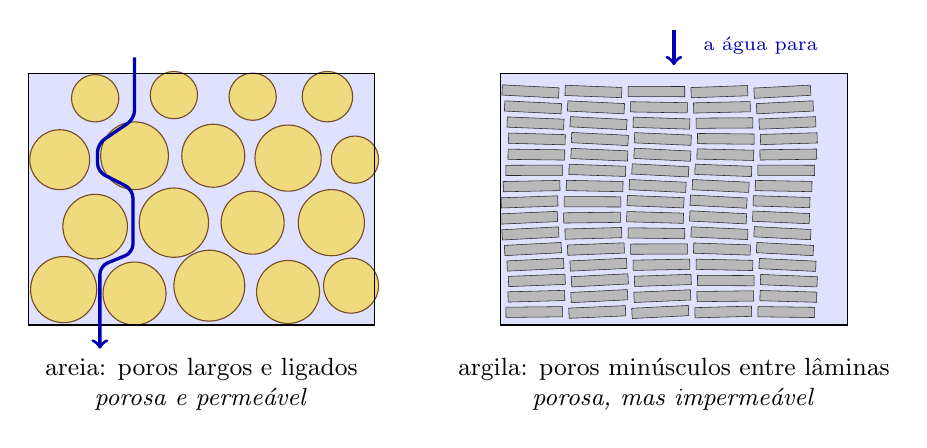
\begin{tikzpicture}
  % sand
  \begin{scope}
    \fill[blue!12] (0,0) rectangle (4.4,3.2);
    \foreach \x/\y/\r in {0.45/0.45/0.42, 1.35/0.4/0.4, 2.3/0.5/0.45, 3.3/0.42/0.4, 4.1/0.5/0.35,
                         0.85/1.25/0.41, 1.85/1.3/0.44, 2.85/1.3/0.4, 3.85/1.3/0.42,
                         0.4/2.1/0.38, 1.35/2.15/0.43, 2.35/2.15/0.4, 3.3/2.12/0.42, 4.15/2.1/0.3,
                         0.85/2.88/0.3, 1.85/2.92/0.3, 2.85/2.9/0.3, 3.8/2.9/0.32}
      \fill[yellow!55!brown!60, draw=brown!60!black] (\x,\y) circle (\r);
    \draw (0,0) rectangle (4.4,3.2);
    \draw[->, blue!70!black, very thick, rounded corners=3pt] (1.35,3.4) -- (1.35,2.62) -- (0.88,2.3) -- (0.88,1.95) -- (1.33,1.72) -- (1.33,0.92) -- (0.91,0.75) -- (0.91,-0.3);
    \node[font=\small, align=center] at (2.2,-0.75) {areia: poros largos e ligados\\ \emph{porosa e permeável}};
  \end{scope}
  % clay
  \begin{scope}[xshift=6.0cm]
    \fill[blue!12] (0,0) rectangle (4.4,3.2);
    \foreach \y in {0.1,0.3,...,3.0}
      \foreach \x in {0.05,0.85,...,3.7}
        \fill[gray!55, draw=gray!30!black, line width=0.2pt, rotate around={{3*sin(57*\x+91*\y)}:(\x+0.36,\y+0.06)}]
          ({\x+0.05*sin(200*\y)},\y) rectangle ++(0.72,0.13);
    \draw (0,0) rectangle (4.4,3.2);
    \draw[->, blue!70!black, very thick] (2.2,3.75) -- (2.2,3.3);
    \node[font=\scriptsize, blue!70!black] at (3.3,3.55) {a água para};
    \node[font=\small, align=center] at (2.2,-0.75) {argila: poros minúsculos entre lâminas\\ \emph{porosa, mas impermeável}};
  \end{scope}
\end{tikzpicture}

{\small Os \omterm{def:g6:water-underground:porosity}{poros} (em azul) entre os grãos de uma \omterm{def:g3:stones-pebbles-sand:sand}{areia} e entre as lâminas
de uma argila, muito ampliados. A água encontra um caminho através da
\omterm{def:g3:stones-pebbles-sand:sand}{areia}; na argila, ela fica presa.}
\end{omfigure}

A tabela dá a \omterm{def:g6:water-underground:porosity}{porosidade} de alguns materiais e a parte da água que sai
deles sozinha quando eles estão cheios de água. O resto fica grudado nos
grãos.

\begin{center}\small
\begin{tabular}{|l|c|c|}
\hline
\textbf{material} & \textbf{\omterm{def:g6:water-underground:porosity}{porosidade} (\%)} & \textbf{água que escoa (\%)} \\
\hline
solo & 55 & 40 \\
argila & 50 & 2 \\
\omterm{def:g3:stones-pebbles-sand:sand}{areia} & 25 & 22 \\
\omterm{def:g3:stones-pebbles-sand:pebble}{cascalho} & 20 & 19 \\
calcário & 20 & 18 \\
arenito & 11 & 6 \\
granito & 0.1 & 0.09 \\
\hline
\end{tabular}
\end{center}
% ledger: heath:porosity

\begin{method}[Quanta água uma rocha guarda?]\label{met:g6:water-underground:volume}
\begin{enumerate}
  \item Encontre o volume da \omterm{def:g3:stones-pebbles-sand:rock}{rocha} (para um bloco: comprimento $\times$
        largura $\times$ altura).
  \item Multiplique pela \omterm{def:g6:water-underground:porosity}{porosidade} e divida por 100: isso é o volume dos
        \omterm{def:g6:water-underground:porosity}{poros}, ou seja, a água que a \omterm{def:g3:stones-pebbles-sand:rock}{rocha} guarda quando está cheia.
  \item Para a água que escoa, use a segunda porcentagem do mesmo jeito.
        (1~metro cúbico é 1000~litros.)
\end{enumerate}
\end{method}

\begin{example}[Um metro cúbico de areia]\label{ex:g6:water-underground:sand}
Um metro cúbico de \omterm{def:g3:stones-pebbles-sand:sand}{areia}, cheio de água, guarda $1000 \times 25 \div 100 =
250$~litros de água nos seus \omterm{def:g6:water-underground:porosity}{poros}. Desses, $1000 \times 22 \div 100 = 220$
litros escoam sozinhos; 30~litros ficam grudados nos grãos. Um metro cúbico
de argila guarda o dobro de água, 500~litros, mas só 20~litros escoam.
% ledger: heath:porosity
\end{example}

\begin{inthelab}[Areia ou argila? (em aula, com a professora)]
Dois vasos de flores com um furo no fundo ficam em cima de dois copos. Um
é cheio de \omterm{def:g3:stones-pebbles-sand:sand}{areia} seca, o outro de terra argilosa seca, bem apertada. A
professora despeja o mesmo copo de água em cada um, ao mesmo tempo. Através
da \omterm{def:g3:stones-pebbles-sand:sand}{areia}, a água logo pinga no copo de baixo. Na argila, a água fica em
cima como uma poça, e só algumas gotas passam, devagar: a \omterm{def:g3:stones-pebbles-sand:sand}{areia} é
\omterm{def:g6:water-underground:permeability}{permeável}, a argila não.
\end{inthelab}

\section{A água subterrânea e o lençol freático}

Cave um buraco na \omterm{def:g3:stones-pebbles-sand:sand}{areia} de uma praia, a alguns passos do \omterm{def:g2:water-on-earth:ocean}{mar}: depois de um
tempinho, a água aparece no fundo do buraco. Você chegou ao lugar onde
todos os \omterm{def:g6:water-underground:porosity}{poros} da \omterm{def:g3:stones-pebbles-sand:sand}{areia} estão cheios de água.
% ledger: wss:aquifer

\begin{definition}[Água subterrânea]\label{def:g6:water-underground:groundwater}
A \emph{água subterrânea}\index{agua subterranea@água subterrânea} é a água embaixo do
chão que enche os \omterm{def:g6:water-underground:porosity}{poros} e as rachaduras do solo e das \omterm{def:g3:stones-pebbles-sand:rock}{rochas}.
\end{definition}

\begin{definition}[Lençol freático]\label{def:g6:water-underground:water-table}
Abaixo de uma certa profundidade, todos os \omterm{def:g6:water-underground:porosity}{poros} da \omterm{def:g3:stones-pebbles-sand:rock}{rocha} estão cheios de
água. O \emph{lençol freático}\index{lencol freatico@lençol freático} é o topo dessa zona cheia de
água. Acima dele, os \omterm{def:g6:water-underground:porosity}{poros} guardam ar e um pouco de água; abaixo dele,
eles estão cheios de água.
% ledger: wss:aquifer
\end{definition}

O \omterm{def:g6:water-underground:water-table}{lençol freático} não é plano. Ele segue a forma do terreno, mas de modo
mais suave: mais alto embaixo dos morros, mais baixo embaixo dos \omterm{def:g1:landscapes-around-us:landform}{vales}.
Ele também sobe e desce com as estações. Depois de uma estação chuvosa, a
\omterm{def:g4:clouds-rain-snow:precipitation}{chuva} que se infiltrou o faz subir; depois de uma longa estação seca, a
água escoa devagar para as \omterm{def:g6:water-underground:spring}{fontes} e os \omterm{def:g1:landscapes-around-us:water}{rios}, e o \omterm{def:g6:water-underground:water-table}{lençol freático} desce.

A \omterm{def:g6:water-underground:groundwater}{água subterrânea} é uma grande reserva de \omterm{def:g2:water-on-earth:salt-fresh}{água doce}. De toda a \omterm{def:g2:water-on-earth:salt-fresh}{água doce}
da Terra, cerca de 69~\% é gelo e \omterm{def:g4:clouds-rain-snow:precipitation}{neve} permanente, e cerca de 30~\% é \omterm{def:g6:water-underground:groundwater}{água
subterrânea}; a \omterm{def:g2:water-on-earth:salt-fresh}{água doce} de todos os \omterm{def:g1:landscapes-around-us:water}{lagos} é só cerca de um quarto de um
por cento. A \omterm{def:g6:water-underground:groundwater}{água subterrânea} é mais de cem vezes mais abundante que a
\omterm{def:g2:water-on-earth:salt-fresh}{água doce} dos \omterm{def:g1:landscapes-around-us:water}{lagos}.
% ledger: wss:fresh-shares

\begin{omfigure}
\begin{tikzpicture}
  \begin{axis}[xbar, width=0.8\linewidth, height=3.9cm, bar width=8pt,
      xmin=0, xmax=85, ymin=-0.6, ymax=4.6, y dir=reverse,
      ytick={0,...,4}, yticklabels={gelo e neve permanente,água subterrânea,gelo do solo e permafrost,lagos,todo o resto},
      xlabel={porcentagem de toda a água doce da Terra},
      axis x line=bottom, axis y line=left, axis line style={-},
      tick label style={font=\scriptsize}, label style={font=\small},
      nodes near coords, nodes near coords style={font=\scriptsize, anchor=west},
      point meta=explicit symbolic, enlarge y limits=false, clip=false]
    \addplot[fill=blue!35, draw=blue!60!black] table[x=pct, y=idx, meta=pct] {figdata/out/grade-6-water_table-fresh.dat};
  \end{axis}
\end{tikzpicture}

{\small Onde fica a \omterm{def:g2:water-on-earth:salt-fresh}{água doce} da Terra. As barras dos \omterm{def:g1:landscapes-around-us:water}{lagos} e de todo o
resto (os \omterm{def:g1:landscapes-around-us:water}{rios}, o ar, o solo, os pântanos, os seres vivos) são curtas
demais para ver.}
% ledger: wss:fresh-shares (figdata/grade-6/water_table.py, part fresh)
\end{omfigure}

\section{Fontes e poços}

\begin{definition}[Fonte e poço]\label{def:g6:water-underground:spring}
Uma \emph{fonte}\index{fonte} é um lugar onde a \omterm{def:g6:water-underground:groundwater}{água subterrânea} sai do chão
sozinha, onde o \omterm{def:g6:water-underground:water-table}{lençol freático} encontra a superfície. Um
\emph{poço}\index{poco@poço} é um buraco cavado ou perfurado até abaixo do
\omterm{def:g6:water-underground:water-table}{lençol freático}, para que a \omterm{def:g6:water-underground:groundwater}{água subterrânea} encha o seu fundo e possa ser
retirada.
\end{definition}

O corte abaixo atravessa um \omterm{def:g1:landscapes-around-us:landform}{vale} das Colinas de Varden, a região dos
nossos exercícios. As \omterm{def:g1:landscapes-around-us:landform}{colinas} são feitas de giz, um calcário branco, mole,
\omterm{def:g6:water-underground:porosity}{poroso} e \omterm{def:g6:water-underground:permeability}{permeável}. Embaixo do giz há uma camada de folhelho, que é
\omterm{def:g6:water-underground:permeability}{impermeável}. A \omterm{def:g4:clouds-rain-snow:precipitation}{chuva} se infiltra no giz, enche os seus \omterm{def:g6:water-underground:porosity}{poros} e para no
folhelho.

\begin{omfigure}
\begin{tikzpicture}
\begin{axis}[omsection, width=0.95\linewidth, height=7.2cm,
    xmin=0, xmax=2.8, ymin=0, ymax=560,
    xlabel={distância desde a ponta sul do corte (km)},
    ylabel={altura acima do nível do mar (m)},
    tick label style={font=\scriptsize}, label style={font=\small},
    clip mode=individual]
  \addplot[om lith={icsJurassic!40}{om limestone}, draw=black, line width=0.3pt, even odd rule] table {figdata/out/grade-6-water_table-unit-limestone.dat};
  \addplot[om lith={icsJurassic!15}{om shale}, draw=black, line width=0.3pt, even odd rule] table {figdata/out/grade-6-water_table-unit-shale.dat};
  \addplot[om lith={icsCretaceous!35}{om limestone}, draw=black, line width=0.3pt, even odd rule] table {figdata/out/grade-6-water_table-unit-chalk.dat};
  \addplot[lith alluvium, draw=black, line width=0.3pt, even odd rule] table {figdata/out/grade-6-water_table-unit-alluvium.dat};
  \addplot[black, thick] table {figdata/out/grade-6-water_table-ground.dat};
  \addplot[blue!75!black, very thick] table {figdata/out/grade-6-water_table-wet.dat};
  \addplot[blue!75!black, very thick, dashed] table {figdata/out/grade-6-water_table-dry.dat};
  % wells
  \addplot[fill=white, draw=black, line width=0.4pt] table {figdata/out/grade-6-water_table-well-rects.dat};
  \addplot[only marks, mark=none, point meta=explicit symbolic, nodes near coords,
    nodes near coords style={font=\scriptsize\bfseries, anchor=south east, fill=white, fill opacity=0.8, text opacity=1, inner sep=1pt}]
    table[x=s_km, y=z_m, meta=label, row sep=\\] {s_km z_m label\\ 1.45 401.3 poço~A\\ 1.7 470.3 poço~B\\ };
  % river and spring
  \addplot[only marks, mark=*, mark size=2.2pt, blue!75!black] table[x=s_km, y=z_m] {figdata/out/grade-6-water_table-points.dat};
  \node[font=\scriptsize, blue!70!black, anchor=south east] at (axis cs:0.215,140) {rio};
  \node[font=\scriptsize, blue!70!black, anchor=east] at (axis cs:0.83,218) {fonte};
  \node[font=\scriptsize] at (axis cs:2.2,470) {giz (permeável)};
  \node[font=\scriptsize, fill=white, fill opacity=0.8, text opacity=1] at (axis cs:2.2,95) {folhelho (impermeável)};
  \node[font=\scriptsize, fill=white, fill opacity=0.8, text opacity=1] at (axis cs:0.95,25) {calcário};
  \node[font=\scriptsize, blue!70!black, fill=white, fill opacity=0.8, text opacity=1, align=center] at (axis cs:2.15,250) {lençol freático:\\ depois da estação chuvosa (contínua)\\ depois da estação seca (tracejada)};
\end{axis}
\end{tikzpicture}

{\small Um corte norte--sul através das Colinas de Varden, do \omterm{def:g1:landscapes-around-us:water}{rio} até o
alto da encosta norte (alturas exageradas cerca de 2~vezes). A água
guardada no giz para no folhelho e sai como uma \omterm{def:g6:water-underground:spring}{fonte} onde a base do giz
encontra a encosta. O \omterm{def:g6:water-underground:spring}{poço}~A sempre alcança a água; o \omterm{def:g6:water-underground:spring}{poço}~B só a alcança
depois da estação chuvosa.}
% (figdata/grade-6/water_table.py; region model figdata/shared/region.py)
\end{omfigure}

A \omterm{def:g6:water-underground:spring}{fonte} corre onde a base do giz encontra a encosta: a água não consegue
descer através do folhelho, então ela corre ao longo do topo do folhelho e
sai na encosta. Enquanto houver água no giz acima do folhelho, a \omterm{def:g6:water-underground:spring}{fonte}
continua correndo, mesmo num verão seco: essa é a resposta à pergunta feita
no começo do capítulo.

Observe os dois \omterm{def:g6:water-underground:spring}{poços}. O \omterm{def:g6:water-underground:spring}{poço}~A tem 100~m de profundidade; o seu fundo fica
abaixo do \omterm{def:g6:water-underground:water-table}{lençol freático} em todas as estações, então ele sempre dá água.
O \omterm{def:g6:water-underground:spring}{poço}~B é ainda mais fundo, 105~m, mas foi cavado mais acima na \omterm{def:g1:landscapes-around-us:landform}{colina}: o
seu fundo fica abaixo do \omterm{def:g6:water-underground:water-table}{lençol freático} depois da estação chuvosa e acima
dele depois da estação seca. No verão, o \omterm{def:g6:water-underground:spring}{poço}~B fica sem água. O que
importa não é a profundidade de um \omterm{def:g6:water-underground:spring}{poço}, mas quanto o seu fundo desce
abaixo do \omterm{def:g6:water-underground:water-table}{lençol freático} mais baixo.
% (figdata/grade-6/water_table.py, part wells)

\begin{omfigure}
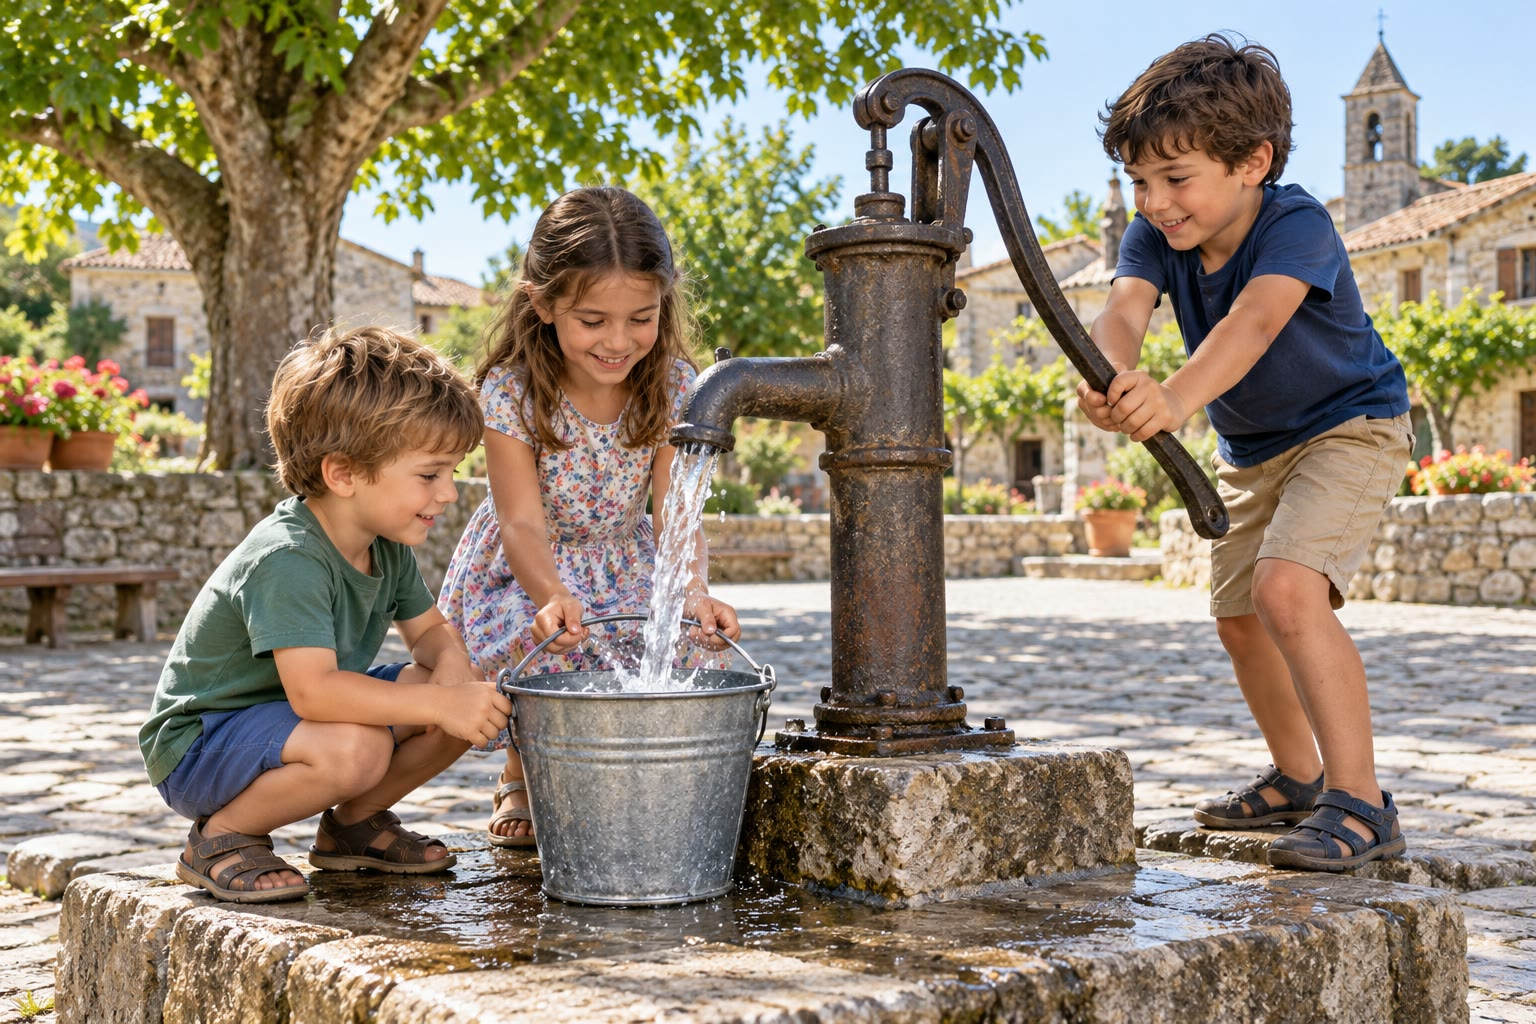
\includegraphics[width=0.6\linewidth]{images/book1/ai/g6-hand-pump.jpg}

{\small Crianças enchem um balde na bomba manual do \omterm{def:g6:water-underground:spring}{poço} de uma aldeia.
(Ilustração feita por IA.)}
\end{omfigure}

\begin{remark}[Um poço pode secar]\label{rem:g6:water-underground:pumping}
Bombear água de um \omterm{def:g6:water-underground:spring}{poço} faz o \omterm{def:g6:water-underground:water-table}{lençol freático} baixar em volta dele. Se a
água for bombeada mais depressa do que a \omterm{def:g4:clouds-rain-snow:precipitation}{chuva} reabastece a \omterm{def:g3:stones-pebbles-sand:rock}{rocha}, o \omterm{def:g6:water-underground:water-table}{lençol
freático} desce cada vez mais: o \omterm{def:g6:water-underground:spring}{poço} dá cada vez menos água e pode secar.
Dois vizinhos que bombeiam da mesma \omterm{def:g3:stones-pebbles-sand:rock}{rocha} dividem a mesma água: uma bomba
pode secar o \omterm{def:g6:water-underground:spring}{poço} do outro.
% ledger: wss:aquifer
\end{remark}

\section{Os aquíferos}

\begin{definition}[Aquífero]\label{def:g6:water-underground:aquifer}
Um \emph{aquífero}\index{aquifero@aquífero} é uma camada de \omterm{def:g3:stones-pebbles-sand:rock}{rocha} \omterm{def:g6:water-underground:porosity}{porosa} e \omterm{def:g6:water-underground:permeability}{permeável},
cheia de \omterm{def:g6:water-underground:groundwater}{água subterrânea}, que deixa essa água escoar até as \omterm{def:g6:water-underground:spring}{fontes} e os
\omterm{def:g6:water-underground:spring}{poços}. A \omterm{def:g4:clouds-rain-snow:precipitation}{chuva} que se infiltra o reabastece.
% ledger: wss:aquifer
\end{definition}

O giz das Colinas de Varden é um \omterm{def:g6:water-underground:aquifer}{aquífero}: ele é \omterm{def:g6:water-underground:porosity}{poroso}, é \omterm{def:g6:water-underground:permeability}{permeável}, e os
sítios das \omterm{def:g1:landscapes-around-us:landform}{colinas} tiram dele a sua água. O folhelho embaixo dele não é um
\omterm{def:g6:water-underground:aquifer}{aquífero}: a água não consegue atravessá-lo. Mais fundo ainda, embaixo do
folhelho, ficam um calcário e um arenito, que também podem guardar água;
para chegar a ela, é preciso perfurar um \omterm{def:g6:water-underground:spring}{poço} através de todo o folhelho.

A \omterm{def:g6:water-underground:groundwater}{água subterrânea} faz parte do ciclo da água. A \omterm{def:g4:clouds-rain-snow:precipitation}{chuva} se infiltra num
\omterm{def:g6:water-underground:aquifer}{aquífero}; a \omterm{def:g6:water-underground:groundwater}{água subterrânea} corre devagar pelos \omterm{def:g6:water-underground:porosity}{poros}; ela sai nas \omterm{def:g6:water-underground:spring}{fontes} e nos \omterm{def:g1:landscapes-around-us:water}{rios}, que a levam até o \omterm{def:g2:water-on-earth:ocean}{mar}; ali
ela evapora e cai de novo como \omterm{def:g4:clouds-rain-snow:precipitation}{chuva}. Tirar água de um \omterm{def:g6:water-underground:aquifer}{aquífero} é como
tirar água de uma caixa d'água que a \omterm{def:g4:clouds-rain-snow:precipitation}{chuva} enche devagar: ela só dura se
não tirarmos mais do que a \omterm{def:g4:clouds-rain-snow:precipitation}{chuva} devolve.

\section{Manter a água subterrânea limpa}

A água que se infiltra no chão é filtrada no caminho: as folhas, as
partículas de solo e os bichinhos ficam retidos pelo solo e pela \omterm{def:g3:stones-pebbles-sand:rock}{rocha}. É
por isso que a água de uma \omterm{def:g6:water-underground:spring}{fonte} ou de um \omterm{def:g6:water-underground:spring}{poço} em geral parece
cristalina. Mas as substâncias \emph{dissolvidas} na água não ficam
retidas: elas descem com ela até o \omterm{def:g6:water-underground:water-table}{lençol freático}.
% ledger: wss:gw-quality

A \omterm{def:g6:water-underground:groundwater}{água subterrânea} pode ser estragada pelo que as pessoas põem no chão: os
fertilizantes e os agrotóxicos espalhados nos campos e nos jardins, o sal
espalhado nas estradas congeladas, o combustível que vaza de um tanque, o
lixo jogado a céu aberto, o transbordamento de fossas malcuidadas das
casas. Depois de dissolvidas num \omterm{def:g6:water-underground:aquifer}{aquífero}, essas substâncias são difíceis
de remover, e a água pode deixar de ser segura para beber sem tratamento. Por isso, a água de um \omterm{def:g6:water-underground:spring}{poço} tem de ser analisada antes de ser bebida, e é melhor manter os fertilizantes, o combustível e o lixo longe dos \omterm{def:g6:water-underground:spring}{poços} e das \omterm{def:g6:water-underground:spring}{fontes}.
% ledger: wss:gw-quality

As substâncias dissolvidas viajam com a \omterm{def:g6:water-underground:groundwater}{água subterrânea}. Abaixo do \omterm{def:g6:water-underground:water-table}{lençol
freático}, a água desliza devagar ladeira abaixo: de onde o \omterm{def:g6:water-underground:water-table}{lençol freático}
é alto, embaixo dos morros, até onde ele é baixo, nas \omterm{def:g6:water-underground:spring}{fontes} e nos \omterm{def:g1:landscapes-around-us:water}{rios}. Um
vazamento que se infiltra, então, não fica onde caiu. Ele afunda até o
\omterm{def:g6:water-underground:water-table}{lençol freático} e depois vai sendo levado ladeira abaixo com a \omterm{def:g6:water-underground:groundwater}{água
subterrânea}, na direção de tudo o que fica abaixo dele na encosta.
% ledger: wss:gw-quality, wss:aquifer

\begin{omfigure}
\begin{tikzpicture}[x=1cm, y=1.15cm, font=\scriptsize]
  % ground (the chalk) and the water-filled zone under the water table
  \fill[black!6] (0,0) -- (0,4.090) -- plot[smooth] coordinates {(0.00,4.090) (1.00,4.013) (2.00,3.887) (3.00,3.692) (4.00,3.407) (5.00,3.033) (6.00,2.600) (7.00,2.167) (8.00,1.793) (9.00,1.508) (10.00,1.313) (11.00,1.187) (12.00,1.110)} -- (12,0) -- cycle;
  \fill[blue!14] (0,0) -- (0,3.190) -- plot[smooth] coordinates {(0.00,3.190) (1.00,3.185) (2.00,3.131) (3.00,3.008) (4.00,2.795) (5.00,2.493) (6.00,2.132) (7.00,1.771) (8.00,1.469) (9.00,1.256) (10.00,1.133) (11.00,1.079) (12.00,1.074)} -- (12,0) -- cycle;
  \draw[black!70, line width=0.7pt] plot[smooth] coordinates {(0.00,4.090) (1.00,4.013) (2.00,3.887) (3.00,3.692) (4.00,3.407) (5.00,3.033) (6.00,2.600) (7.00,2.167) (8.00,1.793) (9.00,1.508) (10.00,1.313) (11.00,1.187) (12.00,1.110)};
  \draw[blue!70!black, dashed, line width=0.7pt] plot[smooth] coordinates {(0.00,3.190) (1.00,3.185) (2.00,3.131) (3.00,3.008) (4.00,2.795) (5.00,2.493) (6.00,2.132) (7.00,1.771) (8.00,1.469) (9.00,1.256) (10.00,1.133) (11.00,1.079) (12.00,1.074)};
  % the spill: down to the water table, then downhill with the groundwater
  \fill[brown!70!black, opacity=0.55] (4.85,3.094) -- (5.15,2.971) -- (5.15,2.442) -- (4.85,2.544) -- cycle;
  \fill[brown!70!black, opacity=0.55] (4.85,2.514) -- (5.10,2.429) -- (5.35,2.341) -- (5.60,2.250) -- (5.85,2.158) -- (6.10,2.065) -- (6.35,1.972) -- (6.60,1.881) -- (6.85,1.792) -- (7.10,1.707) -- (7.35,1.626) -- (7.60,1.549) -- (7.85,1.478) -- (8.10,1.413) -- (8.35,1.354) -- (8.60,1.300) -- (8.85,1.252) -- (9.10,1.210) -- (9.30,1.181) -- (9.10,1.182) -- (8.85,1.190) -- (8.60,1.203) -- (8.35,1.221) -- (8.10,1.246) -- (7.85,1.277) -- (7.60,1.313) -- (7.35,1.355) -- (7.10,1.401) -- (6.85,1.486) -- (6.60,1.598) -- (6.35,1.713) -- (6.10,1.828) -- (5.85,1.945) -- (5.60,2.060) -- (5.35,2.174) -- (5.10,2.286) -- (4.85,2.394) -- cycle;
  % the leaking tank
  \draw[fill=black!35] (4.7,3.10) rectangle (5.3,3.42);
  \node[anchor=south, align=center] at (5.0,3.45) {tanque de\\combustível vazando};
  % groundwater flow
  \begin{scope}[blue!60!black, -{Stealth[length=2mm]}, line width=0.8pt]
    \draw (0.80,2.589) -- (2.40,2.491);
    \draw (3.40,2.334) -- (5.00,1.893);
    \draw (5.90,1.569) -- (7.50,1.009);
    \draw (8.80,0.691) -- (10.60,0.494);
  \end{scope}
  \node[blue!60!black, anchor=north] at (6.7,1.0) {a água subterrânea desce a encosta};
  % the two wells
  \draw[line width=1.6pt, black!75] (2.0,3.887) -- (2.0,2.70);
  \draw[line width=1.6pt, black!75] (8.5,1.639) -- (8.5,0.95);
  \node[anchor=south, align=center] at (2.0,3.95) {poço A\\(acima): limpo};
  \draw[black!50] (8.5,1.66) -- (8.5,2.30);
  \node[anchor=south, align=center] at (8.5,2.30) {poço B\\(abaixo): estragado};
  % the stream
  \fill[blue!60] (11.55,1.13) -- (11.95,1.11) -- (11.75,1.02) -- cycle;
  \node[anchor=south] at (11.6,1.20) {riacho};
  \node[blue!70!black, anchor=south west] at (0.1,3.21) {lençol freático};
  \node[anchor=west, black!70] at (0.15,0.25) {giz};
\end{tikzpicture}

{\small Um vazamento numa encosta (um esboço). O combustível dissolvido
afunda até o \omterm{def:g6:water-underground:water-table}{lençol freático} e depois é levado ladeira abaixo com a \omterm{def:g6:water-underground:groundwater}{água
subterrânea} (setas azuis): ele chega ao \omterm{def:g6:water-underground:spring}{poço} B, abaixo dele na encosta, e
por fim ao riacho. O \omterm{def:g6:water-underground:spring}{poço} A, acima do tanque, continua limpo.}
\end{omfigure}

\begin{method}[Um poço está em risco?]\label{met:g6:water-underground:risk}
\begin{enumerate}
  \item Encontre onde o \omterm{def:g6:water-underground:water-table}{lençol freático} é alto e onde ele é baixo: ele é
        alto embaixo dos morros e baixo perto das \omterm{def:g6:water-underground:spring}{fontes} e dos \omterm{def:g1:landscapes-around-us:water}{rios}.
  \item A \omterm{def:g6:water-underground:groundwater}{água subterrânea} corre do alto para o baixo: desenhe a sua
        direção com uma seta.
  \item Um \omterm{def:g6:water-underground:spring}{poço} ou uma \omterm{def:g6:water-underground:spring}{fonte} que fica abaixo de uma \omterm{def:g6:water-underground:spring}{fonte} de poluição, no
        caminho dessa seta, está em risco; um \omterm{def:g6:water-underground:spring}{poço} acima dela não está.
\end{enumerate}
\end{method}

\begin{example}[Um novo tanque de combustível para o sítio]\label{ex:g6:water-underground:tank}
Uma agricultora, numa encosta de giz, bebe a água do seu próprio \omterm{def:g6:water-underground:spring}{poço}, no
meio da encosta, e quer pôr um novo tanque de combustível num de dois
campos: um acima do \omterm{def:g6:water-underground:spring}{poço}, outro abaixo dele, perto do riacho. A \omterm{def:g6:water-underground:groundwater}{água
subterrânea} desce a encosta. Um vazamento no campo de cima desceria na
direção do \omterm{def:g6:water-underground:spring}{poço}; um vazamento no campo de baixo se afastaria dele, na
direção do riacho. O campo abaixo do \omterm{def:g6:water-underground:spring}{poço} é a melhor escolha para o \omterm{def:g6:water-underground:spring}{poço}
--- e um tanque numa bandeja que segura qualquer vazamento é melhor ainda,
porque o riacho também importa.
\end{example}

\begin{inthefield}[Encontrar fontes]
Num passeio com um adulto, observe o pé de uma encosta. Uma \omterm{def:g6:water-underground:spring}{fonte} muitas
vezes aparece como uma mancha de chão úmido, uma faixa de grama mais verde
ou de juncos num campo seco, um riachinho que começa do nada, ou uma bacia
de pedra ou um bebedouro construído para recolher a água. Num \omterm{def:g2:drawing-to-map:map}{mapa} de
trilhas detalhado, as \omterm{def:g6:water-underground:spring}{fontes} são marcadas com um pequeno símbolo. Observe
da trilha: nunca beba a água de uma \omterm{def:g6:water-underground:spring}{fonte} que não foi analisada.
\end{inthefield}

\section{Exercícios}

\begin{exercise}[$\star$]\label{exo:g6:water-underground:1}
Classifique estes materiais em ``\omterm{def:g6:water-underground:permeability}{permeáveis}'' e ``\omterm{def:g6:water-underground:permeability}{impermeáveis}'': \omterm{def:g3:stones-pebbles-sand:sand}{areia},
argila, \omterm{def:g3:stones-pebbles-sand:pebble}{cascalho}, granito sem rachaduras, folhelho, giz.
\end{exercise}

\begin{exercise}[$\star$]\label{exo:g6:water-underground:2}
Ligue cada palavra ao seu significado: \omterm{def:g6:water-underground:spring}{fonte}; \omterm{def:g6:water-underground:spring}{poço}; \omterm{def:g6:water-underground:water-table}{lençol freático};
\omterm{def:g6:water-underground:aquifer}{aquífero}. (a) O topo da zona em que todos os \omterm{def:g6:water-underground:porosity}{poros} estão cheios de água.
(b) Uma camada \omterm{def:g6:water-underground:porosity}{porosa} e \omterm{def:g6:water-underground:permeability}{permeável} que guarda \omterm{def:g6:water-underground:groundwater}{água subterrânea}. (c) Um
lugar onde a \omterm{def:g6:water-underground:groundwater}{água subterrânea} sai sozinha. (d) Um buraco que desce até
abaixo do \omterm{def:g6:water-underground:water-table}{lençol freático}.
\end{exercise}

\begin{exercise}[$\star$]\label{exo:g6:water-underground:3}
(a) Dê o nome dos três caminhos que a água da \omterm{def:g4:clouds-rain-snow:precipitation}{chuva} pode seguir quando cai
na terra. (b) Depois de uma \omterm{def:g5:natural-hazards:storm}{tempestade}, onde escorre mais água: num
estacionamento ou num prado? Por quê?
\end{exercise}

\begin{exercise}[$\star$]\label{exo:g6:water-underground:4}
Verdadeiro ou falso? Corrija as frases falsas. (a) Uma \omterm{def:g3:stones-pebbles-sand:rock}{rocha} \omterm{def:g6:water-underground:porosity}{porosa} é
sempre \omterm{def:g6:water-underground:permeability}{permeável}. (b) Abaixo do \omterm{def:g6:water-underground:water-table}{lençol freático}, os \omterm{def:g6:water-underground:porosity}{poros} estão cheios de
água. (c) O \omterm{def:g6:water-underground:water-table}{lençol freático} é plano, como a superfície de um \omterm{def:g1:landscapes-around-us:water}{lago}. (d) Há
mais \omterm{def:g2:water-on-earth:salt-fresh}{água doce} embaixo do chão que em todos os \omterm{def:g1:landscapes-around-us:water}{lagos}.
\end{exercise}

\begin{exercise}[$\star\star$]\label{exo:g6:water-underground:5}
Um balde guarda 10~litros de \omterm{def:g3:stones-pebbles-sand:sand}{areia} seca. A \omterm{def:g6:water-underground:porosity}{porosidade} da \omterm{def:g3:stones-pebbles-sand:sand}{areia} é de
25~\%. Quanta água você consegue despejar no balde antes que ele
transborde? Quanta água sairia por um furo no fundo (22~\%)?
\end{exercise}

\begin{exercise}[$\star\star$]\label{exo:g6:water-underground:6}
Um bloco de calcário mede 2~m por 1~m por 1~m. (a) Qual é o seu volume, em
metros cúbicos e em litros? (b) A sua \omterm{def:g6:water-underground:porosity}{porosidade} é de 20~\%: quantos
litros de água ele guarda quando está cheio? (c) Dessa água, 18~\% do
volume escoa. Quantos litros escoam, e quantos ficam grudados?
\end{exercise}

\begin{exercise}[$\star\star$]\label{exo:g6:water-underground:7}
Use o corte através das Colinas de Varden. (a) A que altura fica a \omterm{def:g6:water-underground:spring}{fonte}?
E o \omterm{def:g1:landscapes-around-us:water}{rio}? (b) A \omterm{def:g6:water-underground:spring}{fonte} fica acima ou abaixo do \omterm{def:g1:landscapes-around-us:water}{rio}? Para onde vai a água da
\omterm{def:g6:water-underground:spring}{fonte}? (c) Por que não há \omterm{def:g6:water-underground:spring}{fonte} no meio da encosta de giz?
\end{exercise}

\begin{exercise}[$\star\star$]\label{exo:g6:water-underground:8}
No \omterm{def:g6:water-underground:spring}{poço}~A, o chão está a 401~m; o \omterm{def:g6:water-underground:water-table}{lençol freático} está a 336~m depois da
estação chuvosa e a 314~m depois da estação seca. (a) A que profundidade
abaixo do chão fica a água em cada estação? (b) Quantos metros o \omterm{def:g6:water-underground:water-table}{lençol
freático} desce entre as duas estações?
\end{exercise}

\begin{exercise}[$\star\star$]\label{exo:g6:water-underground:9}
Um agricultor quer um novo \omterm{def:g6:water-underground:spring}{poço} no alto da \omterm{def:g1:landscapes-around-us:landform}{colina}, na ponta direita do
corte. O \omterm{def:g6:water-underground:spring}{poço} deve ser mais fundo ou mais raso que o \omterm{def:g6:water-underground:spring}{poço}~A? Explique com o
\omterm{def:g6:water-underground:water-table}{lençol freático}.
\end{exercise}

\begin{exercise}[$\star\star$]\label{exo:g6:water-underground:10}
Um metro cúbico de argila guarda 500~litros de água, mas só dá 20~litros.
Explique por que um \omterm{def:g6:water-underground:spring}{poço} cavado na argila quase não dá água, embora a
argila esteja cheia dela.
\end{exercise}

\begin{exercise}[$\star\star\star$]\label{exo:g6:water-underground:11}
De toda a \omterm{def:g2:water-on-earth:salt-fresh}{água doce} da Terra, 30.1~\% é \omterm{def:g6:water-underground:groundwater}{água subterrânea} e 0.26~\% está
nos \omterm{def:g1:landscapes-around-us:water}{lagos}. (a) Quantas vezes há mais \omterm{def:g2:water-on-earth:salt-fresh}{água doce} embaixo do chão que nos
\omterm{def:g1:landscapes-around-us:water}{lagos}? (b) De toda a \omterm{def:g2:water-on-earth:salt-fresh}{água doce}, cerca de 69~\% é gelo e \omterm{def:g4:clouds-rain-snow:precipitation}{neve}. Que parte
sobra para todo o resto (\omterm{def:g6:water-underground:groundwater}{água subterrânea}, \omterm{def:g1:landscapes-around-us:water}{lagos}, \omterm{def:g1:landscapes-around-us:water}{rios}, o ar, o
solo\ldots)? (c) Por que a \omterm{def:g6:water-underground:groundwater}{água subterrânea} é tão importante para a água
de beber?
\end{exercise}

\begin{exercise}[$\star\star\star$]\label{exo:g6:water-underground:12}
Dois sítios ficam lado a lado sobre o mesmo giz. Num verão, o primeiro
sítio instala uma bomba potente e enche um grande açude; algumas semanas
depois, o \omterm{def:g6:water-underground:spring}{poço} do segundo sítio seca, embora ninguém tenha mexido nele.
Explique o que aconteceu, e o que os dois agricultores poderiam fazer.
\end{exercise}

\section{Problema: O poço do sítio das Colinas de Varden}

\begin{problem}[{Problema de fim de semana --- as rochas embaixo de um
sítio das Colinas de Varden, a água guardada no seu giz e quantos dias ela
duraria sem chuva}]
\label{pb:g6:water-underground:1}
% ledger: heath:porosity, wss:aquifer
Um sítio das Colinas de Varden fica sobre o giz, ao lado do \omterm{def:g6:water-underground:spring}{poço}~A do
corte. O agricultor quer saber por quanto tempo o \omterm{def:g6:water-underground:spring}{poço} conseguiria
abastecer o sítio numa \omterm{def:g5:natural-hazards:drought}{longa seca}, se nenhuma \omterm{def:g4:clouds-rain-snow:precipitation}{chuva} viesse reabastecer
o giz.

\medskip
\noindent\textbf{Parte I --- As rochas embaixo do sítio.}
\begin{enumerate}
  \item Dê o nome da \omterm{def:g3:stones-pebbles-sand:rock}{rocha} sobre a qual o sítio fica e da \omterm{def:g3:stones-pebbles-sand:rock}{rocha} embaixo
        dela. Qual delas é \omterm{def:g6:water-underground:permeability}{permeável}?
  \item Explique por que uma \omterm{def:g6:water-underground:spring}{fonte} corre no pé da encosta abaixo do sítio.
  \item Use o corte: o chão do sítio está a 401~m, e o \omterm{def:g6:water-underground:water-table}{lençol freático}
        está a 336~m depois da estação chuvosa. A que profundidade fica a
        água?
  \item Depois da estação seca, o \omterm{def:g6:water-underground:water-table}{lençol freático} fica a 314~m. O \omterm{def:g6:water-underground:spring}{poço}~A
        tem 100~m de profundidade. Ele ainda alcança a água? Por quantos
        metros?
\end{enumerate}

\medskip
\noindent\textbf{Parte II --- A água no giz.}
O agricultor pode drenar o giz em volta do \omterm{def:g6:water-underground:spring}{poço} num bloco de 100~m de
comprimento, 50~m de largura e 2~m de espessura, abaixo do \omterm{def:g6:water-underground:water-table}{lençol
freático}. O giz é um calcário: use uma \omterm{def:g6:water-underground:porosity}{porosidade} de 20~\% e uma parte de
água que escoa de 18~\%.
\begin{enumerate}[resume]
  \item Qual é o volume do bloco, em metros cúbicos?
  \item Quantos metros cúbicos de água enchem os seus \omterm{def:g6:water-underground:porosity}{poros}?
  \item Quantos metros cúbicos de água escoam dele para o \omterm{def:g6:water-underground:spring}{poço}? Quantos
        ficam presos no giz?
  \item Escreva em litros a água que escoa.
\end{enumerate}

\medskip
\noindent\textbf{Parte III --- Quanto tempo ela dura.}
\begin{enumerate}[resume]
  \item O sítio (casa, animais e horta) usa 18~metros cúbicos de água por
        dia. Quantos litros são?
  \item Quanta água o sítio usa numa semana?
  \item Por que a reserva de água do giz não se esgota num ano normal?
  \item Sem nenhuma \omterm{def:g4:clouds-rain-snow:precipitation}{chuva}, durante quantos dias a água que escoa do bloco
        abasteceria o sítio?
\end{enumerate}
\end{problem}
